\chapter{Analysis}

\section{Introduction}

\subsection{Client Identification}
The client is Ali Woollatt; she is 55 and she has quite high experience with computers. Her job involves using LaTeX to edit documents (usually scientific papers), and as well she uses computers a lot for email, so overall she is very good at understanding computers.

She would like to have an application made for her whereby she is able to calculate and work out her BMI from giving the program her height and BMI, and use this data to try and reach a healthy and optimal weight. Currently she doesn't have any other program to work this out for her, as she doesn't have a smart phone and as a result it means that she can't update on the go. As most applications for weight loss are on smart phones, and the fact that she's not prepared to go out of her way to buy a smart phone just for this one program, she feels that she should be using her personal computer as she uses it for work anyway, she will easily be able to access it. She wants an application that focuses primarily on the BMI but will also display the weight, as well as show her how far she is to achieving her weight loss goal in terms of weeks (e.g. if she is losing at an average rate, it will predict what date she would likely reach her target BMI by if she stayed on course).

She complains about the customization in most health applications, and the fact that there's nothing that she's found where she can create foods/exercises for the database and be able to specify how much exercise she did exactly, which is why she wants an application developed on the computer which will allow for almost full control for the user of their daily routine.

\subsection{Define the current system}
The current system is her having to weight herself every time, and having to calculate the BMI manually. She often has to try and remember the foods/drinks she's had, and work out the calorie intake of each one, and as well try and work out the conversion of calories into grams. This same thing will happen for exercise as well. In the case for walking, if Ali wanted to calculate how many calories she had burnt off, she would use a pedometer which counts the number of steps taken exactly. These steps can then be converted into calories using a calculation and then into grams (1 gram is 9 calories) and kilograms (see volumetrics).

She weights herself using a normal weighing scale, and usually measures her weight in kilograms, and her height in meters. The current system has worked before but has not worked to full effect, as she stopped counting the number of calories taken in and out of her body. Most of this data wasn't written down and instead done mentally, so there was no complete database of what changes were made, and no graph to show her her progress visually.

\subsection{Describe the problems}
There are a lot of problems with this system which are all very serious concerns and extremely important if they are ever going to go into an application. The first major problem is the amount of time this can take, as you often have to be looking at every single item and calculating it individually, meaning time that could've been spent working was spent on tedious calculations. As well as this, it can often be very easily to miss something or to get a piece of data completely wrong, which could make all of the data unreliable.

The second problem with the current system is there is no way of knowing if the data is correct if Ali accidentally makes a human error and does a mis-calculation. this would mean that she gets a piece of bad data, and sometimes she may not even know that she's got the wrong data, which is something that a computer can fix as it already has the steps to complete this action.

The final problem with the current system is that it is hard to track weight over a long period of time to see if the data is accurate.This is a problem for most human as they are prone to forgetting and most have a short term memory when it comes to data, whereas a computer doesn't lose the data. Because of this, if you are going to try to lose weight, it is vitally important that you know if you're on track so you know if you're doing the right thing, which is something that is quite hard to for a human.

\subsection{Section appendix}

%--------------------------------------------------------------------
%Interviewer Questions to client

\subsection{Questions asked to the client}

\subsubsection{Objectives: What is the proposed system to do?}
The overall aim is to help the client maintain a healthy lifestyle by calculating her calorific input and output, and to enable her to lose weight at a sensible (pre-determined) rate. The client is looking at losing 0.5kg/week ($\equiv 3850$kcal/week) but this should be variable.

Once she has reached her target weight, she can continue to use the system to maintain it. An additional calculation of the client's body mass index (BMI) should also be calculated, bearing in mind that a value of between 18.5 and 25 is considered normal.

\subsubsection{What data or information is to be recorded in the proposed system? How much data will the proposed system record?}
The client's height, current weight and target weight will need to be recorded once, at the beginning, together with a sensible weight-loss rate. The app will then calculate how many kcal she needs to `burn' every day. Thereafter, the client needs to be able to input her weight on a weekly basis.

Data for calorific input to be recorded without too much thought. So the client will just say for lunch she had 1 slice brown toast, boiled egg, Kit Kat, white coffee – and the app will know roughly how many calories without her having to weigh everything. 

Data for exercise to be recorded. For sport, she keys in how many hours of tennis (doubles) or cycling, etc., and how many steps she's taken (she's wearing a pedometer); the app then calculates how many calories she has burned.

\subsubsection{How frequently will the data need to be updated?}
It would be useful to input the data as the day progresses. If the app isn't immediately available, she'll need to keep a notebook and update the app each evening. A daily total of $\pm$ kcal will keep her motivated, and all daily records should be kept.

\subsubsection{Will new records need to be added or old ones deleted? How often?}
Only new records will need to be added, preferably daily.

\subsubsection{How important is the data or information that is recorded?}
It's absolutely vital: if the data is not recorded in full there will be no point in the app.

\subsubsection{What processes or functions are to be performed by the new system?}
The system will need a database of the food regularly eaten by the client, which she needs to be able to add to herself. This will contain food types and their calorific content per 100g, and how many grams comprise a `portion'. 

The exercise part also requires a database of the exercise regularly taken by the client; again, she needs to have sufficient access to add activities to this herself. This would contain data for the various activities, and a rough calorie-burning rate.

The system will need to calculate the maximum daily kcal intake allowed (for example, this would be 2000kcal (for a woman) 
minus $(3850\div 7)$kcal), then display what's shown in the `App output' table at the end of this document.

\subsubsection{When should they be done and where?}
The first item (Daily net kcal intake) in the App output table should be instantaneous.

\subsubsection{Are hard copies required?}
No.

\subsubsection{What computing resources does the client possess?}
Smartphone and desktop PC.

\subsubsection{Is the client prepared to purchase hardware/software resources?}
Yes. Will need to purchase a pedometer.

\subsubsection{Is security an issue?}
No.

\subsubsection{Are there any constraints on hardware, software, data, methods of working, cost, time, etc.?}
No.

\subsubsection{Does the user have a particular solution in mind?}
No.
\newpage

\section{Summary}
\begin{table}[h]
\begin{tabular}{lll}
\textbf{User input}\\
\hline\hline
Initial data & Examples of daily input & Weekly input\\
\hline
Height\\
Current weight\\
Target weight\\
Preferred weight-loss rate\\
\hline
& Slice of brown toast\\
& Boiled egg\\
& Kit Kat\\
& White coffee\\
\hline
& Tennis (doubles) 2 hours\\
& Steps 6000\\
\hline
&& Actual weight\\
\hline\hline
\end{tabular}
\vspace{3\baselineskip}

\begin{tabular}{r@{\hspace{5pt}}l}
\textbf{App output}\\
\hline\hline
Daily:  & Net kcal intake above or below the allowed value (below would be negative)\\[6pt]
\multicolumn{2}{l}{The following to be calculated after the weekly weigh-in:}\\[6pt]
Weekly: & How many kcal she was over/under for the week\\[0pt]
Weekly: & BMI\\[0pt]
Weekly: & Total weight loss to date\\[0pt]
Weekly: & Number of days before reaching target weight, at prescribed weight-loss rate\\
\hline\hline
\end{tabular}
\end{table}

%--------------------------------------------------------------------

\section{Investigation}

\subsection{The current system}

\subsubsection{Data sources and destinations}
In the current system, there is only ever 1 primary data source which is Ali herself. This is because she isn't relying on other people to measure her BMI and she is able to get all the data herself without the need for anyone else. Although the data used is only from Ali, you could also mention that Ali uses her own sources from external sources such as her pedometer which she uses and in turn converts into calories, and her weighing scale. Ali would usually do most of the calculations using a calculator as they are easier and more practical to do than just using paper.

The first output for this system is Ali's total calorie count. This data is then processed into the second output, which becomes the total grams lost or gained as a result. This calorie counting is only for helping to predict the data, but Ali may also want to look at her real weight, in which case she uses a weighing scale. The source is the weighing scale which outputs her weight, and as a result she then uses this output to calculate her actual BMI. The destination for all of Ali's data is back to herself, but she is gives the data and returns it back to herself as a different and more useful value.

%---The rest is on a LibreOffice Draw Document---

\includegraphics[width=\textwidth]{CurrentSystemDataSourcesAndDestination.eps}

\subsubsection{Algorithms}
In the current system, there are only a couple of main algorithms being used. One is checking the calories that exist in the foods that have been eaten. The second is checking the calories in the exercise that have been burnt away. The final algorithm is being able to check the BMI of the individual.

The first is calculating food calories:

Total Calories = 0
FOR (food in list) DO
	Total calories = Total Calories + (calories in food) * quantity
END FOR

The second is calculating the calories burnt off with exercise (this can go before or after the food calories. The order doesn't matter as long as you mention Total Calories is 0 at the beginning):

FOR (exercise in list) DO
	Total Calories = Total Calories - (calories in exercise) * quantity
END FOR

The third algorithm is converting the calories into kilograms, and then finally BMI:

Weight in Grams <- Total Calories divided by 9
Weight in kg <- Weight in Grams divided by 1000
BMI = Weight in kg divided by (Height * Height)

\subsubsection{Data flow diagram}
%---It is on a LibreOffice Draw Document---

\subsubsection{Input Forms, Output Forms, Report Formats}
%---I need the client for this one, as Ali isn't reachable right now---

\subsection{The proposed system}

\subsubsection{Data sources and destinations}
%---It is on a LibreOffice Draw Document---

\subsubsection{Data flow diagram}
%---It is on a LibreOffice Draw Document---

\subsubsection{Data dictionary}
%---It is on a LibreOffice Draw Document---

\subsubsection{Volumetrics}
For this system, Ali has said that she only wants it to have the system work for her, and as a result it only needs to have 1 client record. She also chose to have only 1 client due to the fact that it is her work computer, and as a result she's the only person who will be using the desktop at any time, making the idea of extra accounts on the application redundant.

When Ali is using the proposed application, it is important that she enters the data for all her food and exercise on a regular basis, as if she enters a weeks worth of data in just 1 day, it may appear that she's eaten lots during on that one day, and as a result it may make the data harder to understand. As well as this, Ali will have the ability to input her current weight at any time, but it is recommended that she puts it in once every week. This is because the application will be using her actual weight and her predicted weight and comparing them to find out when approximately she will have reached her healthy BMI.

Both the food and exercise databases will come equiped with 10 different objects in each database. This can be increased or decreased, and Ali is able to edit the name/calories of each one. The data kept for each object in the database will be its ID, name and calories. The quantity doesn't need to be kept in a database as the quantity starts off at 1 and the user changes the quantity in the application itself.

As for the amount of data held in the program with regards to extra files, the program will start with:

\begin{itemize}
\item 1 file for Ali's data
\item 10 files for food data
\item 10 files for exercise data
\end{itemize}

All of these files are to hold minimal amounts of data, each worth 1KB each. This means that when the program is first used, it will have 21KB worth of data. But because the program allows for the function of adding and deleting data, this will mean that the total that may be possilbe is higher than 21KB. As I have written in the proposed system data dictionary, the maximum number of foods and exercise are 400 of each, which means 801KB of total data for food, exercise and user data. As for a minimum, I have said the minimum for food and exercise in the proposed system is 1 file for each, meaning the minimum data storage will be 3KB. This amount of data should be no significant problem for Ali's computer, as they are such small amounts of data.
%-----------------------------------------------------------------------------

\section{Objectives}

\subsection{General Objectives}

\begin{itemize}
\item Provide an application that simplifies the process of weight tracking and weight loss
\item Create an optimal and healthy weight for the client
\item Ensure that the client ends up with an optimal BMI
\item Ensure that the BMI predictions will be similar with what the client is meant to be doing
\item Simplified layout
\item Easy to understand data written in a user friendly interface
\end{itemize}

\subsection{Specific Objectives}
Food/Exercise data display:

\begin{itemize}
\item When requested, be able to display any previous client data
\item Simple buttons and layout 
\end{itemize}

Client input
\begin{itemize}
\item Minimal button presses to reach desired location
\item Informative and minimal description on buttons
\item Search bar for adding food/exercise
\end{itemize}

Additional data:
\begin{itemize}
\item Add salt/sugar/fat content for foods
\item Add the quality of the exercise
\item Ability to convert units from metric to industrial
\end{itemize}

Graphs:
\begin{itemize}
\item Easy to read graphs on BMI and weight
\item Ability to show graphs over a specified period of time (e.g. 20 days)
\end{itemize}

\subsection{Core Objectives}

\begin{itemize}
\item Food/Exercise data display
\item Food/Exercise input
\end{itemize}

\subsection{Other Objectives}

\begin{itemize}
\item Graph
\item More food/exercise data
\end{itemize}

%------------------------------------------------------

\section{ER Diagrams and Descriptions}

\subsection{ER Diagram}
%---There is a LibreOffice Document for it---

\subsection{Entity Descriptions}

\begin{itemize}
\item User(Forename, Surname, Height, CurrentWeight, BMI, DesiredWeight, CaloriesPerDay, FoodID, ExerciseID)
\item Food(FoodID, Name, Calories, Quantity)
\item Exercise(ExerciseID, Name, Calories, Time)
\end{itemize}

\section{Object Analysis}

\subsection{Object Listing}

\begin{itemize}
\item User
\item Food
\item Exercise
\end{itemize}

\subsection{Relationship diagrams}
%---There will be LibreOffice Document for it---

\section{Other Abstractions and Graphs}

%------------------------------------------------------

\section{Constraints}

\subsection{Hardware}
Currently Ali uses her computer for all of her online and work related items. She uses 2 Desktop Computers primarily to make editing jobs easier. The new system will need to be able to run on this machine.

Computer Specification:

\begin{itemize}
\item 2 screens: a 28" Display and a 14" Display
\item Intel Core i5-4570 3.2 GHz QuadCore
\item 8GB RAM
\item ASUS H97M-E
\item 120 GB SSD
\item NVIDIA Quadro K600 (1 GB RAM)
\end{itemize}

Due to the computer being so powerful, and the demands of the application being very minimal, the proposed system should more than likely meet the system requirement. The only issue with the hardware isn't an issue of computing power, but due to it being a desktop computer, the system will be constrained to where Ali chooses to have ths system. As well as this, because the computer isn't a laptop, there must be a constant power source for the computer to run as the desktop doesn't have a battery.

\subsection{Software}
Ali has no desired software preference for what can or can't be used, just as long as it gets the job done. Being used on her work computer however, she would like the software to not interfere with the computer, as it has her work documents on them for many clients, and so as a result the only software guideline is that it must work with the current system that Ali already has installed on the computer: Windows 7.

\subsection{Time}
There is no deadline on time set by Ali, but only a deadline set by my teacher. She doesn't need the system in a hurry and is willing to wait until the end of the assignment. As well as this, she would be OK using the program in its prototype form if it is finished earlier than expected.

\subsection{User Knowledge}
If the system all goes to plan with the program built around an easy-to-use user interface, Ali won't need a guide on the program, and she won't even need any experience on most programs to use the application. But seeing as her job is orientated around using LaTeX, and as she uses email regularly, there shouldn't be any serious learning curb with the system, and so as a result, I won't include a user manual for the client.

\subsection{Access restrictions}
Ali has told me that the application does not need to contain any specific access restrictions as such. As this program isn't connected to the internet, and since Ali has told me she's not worried about the type of data that she is holding on the program, due to it being less important, as a result she says that a password protected application is unnecessary and as a result the proposed system is unlikely to have any serious protection.

%---------------------------------------------------

\section{Limitations}

\subsection{Areas which will not be included in computerization}
Anything that Ali inputs into the system is an area that she wasn't originally using computerization for. She completes an activity or eats a food, then she inputs this into the computer to then calculate, but the original activity wouldn't be computerized.

\subsection{Areas considered for future computerization}
As this program isn't sending automated emails, and since the only direction of data is input, there is no other areas that have been considered for computerization.

%---------------------------------------------------

\section{Solutions}

\subsection{Alternative solutions}

\begin{enumerate}
\item Custom Spread Sheet: The advantages of having a custom spread sheet is that they are very readily available on almost any computer, such as Microsoft Excel. This means that no additional software is required for the data. But the disadvantage of this is that although it may have the data, it may not be able to cater for all Ali's needs. As well, the user-interface may suffer as the potential library of data expands.

\item smart phone Application: The advantages of having a BMI tracker on your smart phone are huge. The main reason is that you can add data anywhere you are onto the phone without needing a computer anywhere in sight. As well, for a program like this, a smart phone should be able to handle the processing power and space needed to run the program. But the main disadvantage to this would be that Ali doesn't have a smart phone so because I am specifying this product for the client, due to them not having a smart phone, I cannot code the program for a smart phone. As well, even if Ali did have a smart phone, I would have to edit the coding for the program from computer to a smart phone language, which I have limited knowledge of. As well, the formatting would be different for mobile devices and probably quite hard to grasp.

\item Web Based Application: The advantages of having this on the Internet is that Ali can access it at any time any place as long as she has a reliable Internet connection. As well, it could have an implemented cloud-based system whereby backups exist online. The main disadvantage to having this is that more security is needed as a result of it being online. As well, if the data on weight and BMI is stolen, that is theft of personal data. Being online, it may also make the coding a lot more complex as you have to adjust your coding to web browsers (topics we aren't experts on). Finally, web hosting costs money and may end up costing a lot.

\item Command-line Application: the advantages are it's easier to design and program, and it would be much more efficient in terms of speed and system-resources, making it the fastest running program. As well, the data can be displayed very quickly if Ali has the knowledge. Unfortunately there are a lot of disadvantages, mainly being that a lot of training would be required to use each command, and Ali isn't very knowledgeable on using command lines. As well, it isn't user-friendly due to long lines having to be typed out. Also there are often hidden commands that the client is unaware of, which may result in some data becoming redundant as Ali is unable to find and use it.  Finally a lot more error checking would have to be done for the command-line application, as there is no restriction on what the user can enter.

\item Python Desktop Application with a GUI: The advantages of this is that very little training is needed for the client using the application. The second advantage is the client is able to design the layout and design of the program to be more personal, as well as use features such as radio buttons to compress many processes into 1 action, which results in minimal errors. As well, it can be easy to view large amounts of data. But the main disadvantage is that a lot more time would be needed to create a GUI application as oppose to a Command driven interface. As well, the processing power is likely to be higher for an application run this way than many of the other ways.
\end{enumerate}

\subsection{Justification of chosen solution}
I have chosen to use the "Python Desktop Application with a GUI" solution.
Here are the reasons why I didn't choose the alternative solutions:

\begin{itemize}
\item As the program is designed for only one client,  it means that my program will be specific to that client only and will evolve around her (unlike spread sheets).
\item As Ali doesn't own a smart phone, and is not planning on getting one in the near future, it is redundant to create an application specific for her that works on a device that she doesn't own.
\item The application doesn't require any Internet or WiFi connections to run or help run, and as a result trying to implement a website into the coding would confuse the system entirely. As well, having the application run on a website is redundant because the program only needs to be accessible at home.
\item Trying to use the Command line for the application would've been a disaster, as it would've meant that Ali would've had to learn how to use the command, taking the whole idea away from a friendly user interface.
\end{itemize}

And here are the reasons that I chose to use the "Python Desktop Application with a GUI" solution:

\begin{itemize}
\item I already have a relatively good understanding of the Python language having used it for over a year, and as a result it would be the easiest programming language to code with. As well, I have a limited knowledge of other programming languages
\item It is easier to backup and restore data if the application is a desktop application as it can be saved on your hard drive or external drive
\item My client doesn't need an Internet connection, and wants an easy-to-use interface which adapts, and so having program in the form of a desktop application makes it easier
\end{itemize}